\documentclass[final,t,overlay]{beamer}
\mode<presentation>
{
  \usetheme{UCL}
}
\usepackage[size=a0,scale=1,debug]{beamerposter}

% additional packages
\usepackage[english]{babel}
\usepackage[utf8]{inputenc}
\usepackage{pstool}
\usepackage{calc}
\usepackage{import}
\usepackage{color}
\usepackage{multicol}
\usepackage{graphicx}
\usepackage{tikz}
\usepackage{amsmath}
\usepackage{amsthm,amsthm}
\usepackage{amssymb}
\usetikzlibrary{arrows,shapes}
\tikzstyle{square}=[draw, minimum size=2.5em]
\tikzstyle{round}=[draw,circle, minimum size=2.5em]

 \def\mm#1{\ensuremath{\boldsymbol{#1}}} % version: amsmath
 
\DeclareMathOperator{\diag}{diag}
\DeclareMathOperator{\var}{var}
\DeclareMathOperator{\med}{Median}
\DeclareMathOperator{\chol}{cholesky}
\DeclareMathOperator{\tr}{tr}
\DeclareMathOperator*{\minimise}{minimise}
\DeclareMathOperator*{\argmax}{arg\,max}
\DeclareMathOperator*{\argmin}{arg\,min}

\global\long\def\Mz{M_{\mathbf{z},y}}
\global\long\def\muz{\mu_{\mathbf{z}}}
\global\long\def\aj{\alpha^{(j)}}
\global\long\def\ajt{\left(\alpha^{(j)}\right)^{\top}}

%empf is red now
%\renewcommand{\emph}[1]{{\color{red}{#1}}}

\title{A Kernel Test of Goodness of Fit}
\author[SHORTAUTHOR]
{Kacper Chwialkowski$^*$ Heiko Strathmann$^*$ Arthur Gretton}
\institute[SHORTINSTITUTE]{Gatsby Unit, University College London.}

\date[SHORTDATE]{DATE}

\global\long\def\ev{\mathbb{E}}

\newtheorem{thm}{Theorem}
\definecolor{mg}{rgb}{0,0.44,0}
\usepackage{graphicx}


\begin{document}
\begin{frame}
\begin{columns}
\begin{column}{.33\linewidth}
%\vspace{-0.75cm}
\begin{block}{Motivation: One sample testing for non i.i.d.\ data}
\begin{minipage}{.49\linewidth}

\begin{align*}
 \theta_{1}&\sim{\cal N}(0,10);\theta_{2}\sim{\cal N}(0,1) \\
 X_{i} &\sim\frac{1}{2}{\cal N}(\theta_{1},4)+\frac{1}{2}{\cal N}(\theta_{1}+\theta_{2},4)
\end{align*}
 \vspace{1cm} 

And so we turn the Bayesian crank  to  obtain samples form the posteriori distribution. It obviously matters which matter which method we use, since quality of sample depends on it. 
\end{minipage}
\begin{minipage}{.4\linewidth}
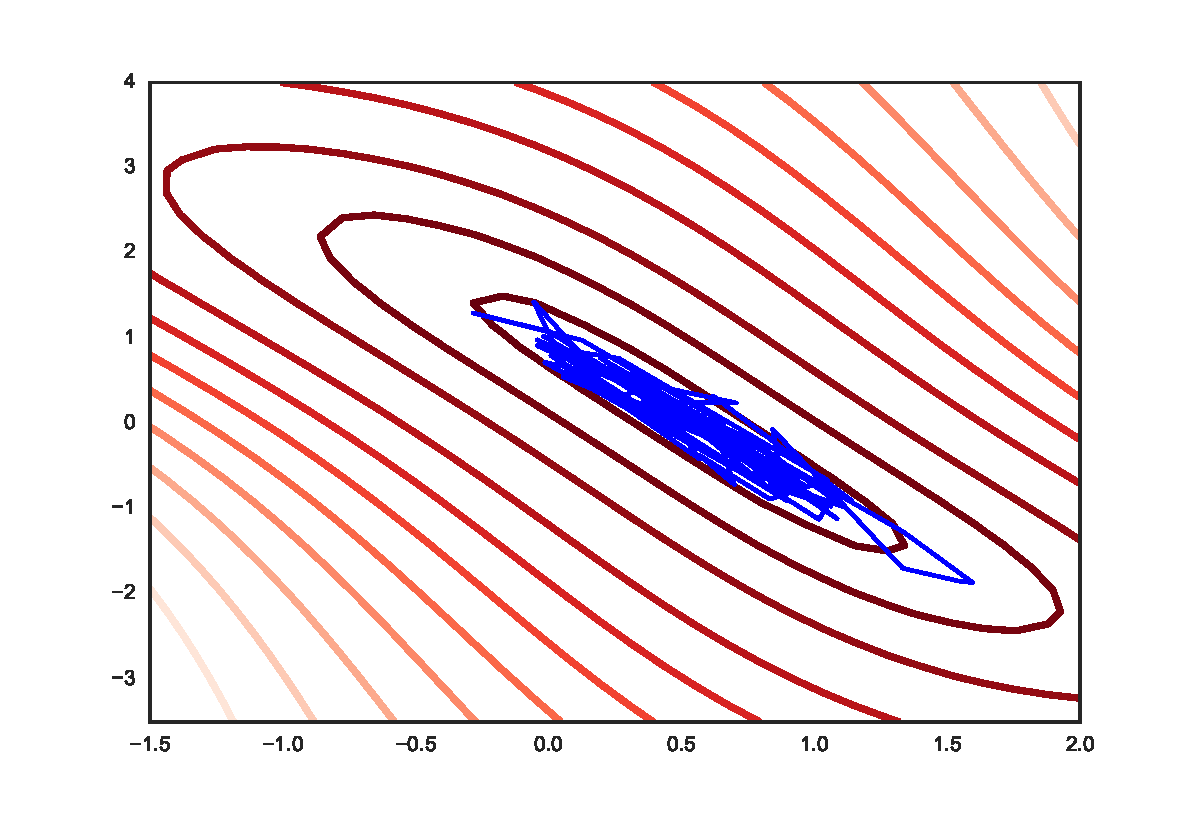
\includegraphics[scale=0.7]{../../presentation/img/sgld_trace_and_density.pdf}
\end{minipage}
\vspace{1cm}
\begin{center}
\Large
\emph{How to check if we sampled from the stationary distribution?}
\end{center}
\end{block}
\vspace{-0.75cm}
\begin{block}{So far: Maximum mean discrepancy}
\begin{center}We turn the kernel crank, we find a function in RKHS to reveal difference in distributions\end{center}
See also \cite{gretton2012kernel}
\begin{minipage}{.60\linewidth}


\vspace{1cm}
\large
\begin{align*}
MMD({\color{red} p},{ \color{blue} q},\mathcal{F}) = \sup_{   \| {\color{mg}f} \|_\mathcal{F}<1} [\ev_{{ \color{blue} q}}{\color{mg}f}- \ev_{{\color{red} p}}{\color{mg} f}]   
\end{align*}
\normalsize
\vspace{1cm}
 \begin{itemize}
  \item $\mathcal{F}$ is an Reproducing kernel Hilbert space.
  \item ${\color{mg} f^*}$ is the function that attains the supremum.
  \item We want to get rid of  $\ev_{ {\color{red} p} }f$ . How?
 \end{itemize}

\end{minipage}
\begin{minipage}{.35\linewidth}

\begin{center}
\vspace{-1cm}
\hspace{-2.5cm}
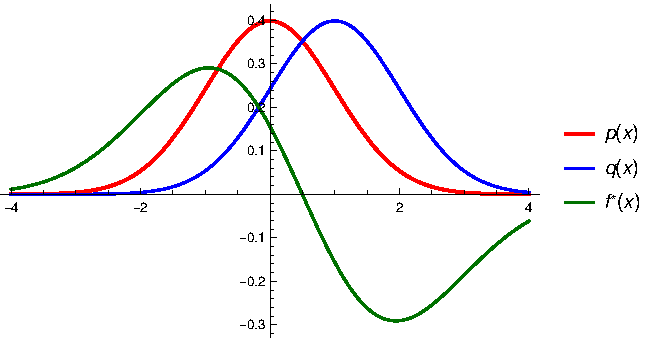
\includegraphics[width=12cm,height=6cm]{../../presentation/img/mmd.pdf}
\end{center}
\end{minipage}
\vspace{1cm}
\begin{center}
\emph{Can we do this without sampling from ${ \color{red} p}$?}
\end{center}
\end{block}
\vspace{-0.75cm}
\begin{block}{Stein's trick in RKHS}

Consider the  class \large
$$G = \{ f  +  \log' { \color{red} p} \cdot  f | f \in \mathcal{F} \}$$
\normalsize
justified by integration by parts
\begin{align*}
 0= &  f(x) {\color{red} p}(x)  \big|_{x=-\infty}^{x=\infty} \\
   = &  \int_{-\infty}^{\infty} (f(x) {\color{red} p}(x) )'  dx \\
   = &  \int   f(x)' { \color{red} p}(x)   + f(x){\color{red} p}'(x)  \\
   = &  \ev_{\color{red} p} f(X)  +  \log' {\color{red} p}(X) f(X) \\
   = & \ev_{\color{red} p} g(X), \\
    & \quad \quad \quad  \quad  \text{ where } g \in G
\end{align*}
With an aid of the Stein operator 
\[
 T_{{ \color{red} p}}f =  f  +  \log' { \color{red} p} \cdot  f
\]
the function class is $G = \{ T_{{ \color{red} p}}f | f \in \mathcal{F} \}$.
Inspired by \cite{gorham2015measuring}, related to \cite{OatGirCho15}, and independently developed in \cite{LiuLeeJor16}.
\end{block}
\vspace{-0.75cm}

\begin{block}{Stein discrepancy}
\large
\begin{align*}
MMD({\color{red} p},{ \color{blue} q},G) = \sup_{   \| {\color{mg} g} \|_G<1} \ev_{{ \color{blue} q}}{\color{mg}g} - \ev_{{\color{red} p}} {\color{mg}g}  = \sup_{ \| {\color{mg} g} \|_G<1} \ev_{{ \color{blue} q}} {\color{mg}g} 
\end{align*}
\vspace{2cm}
\centering
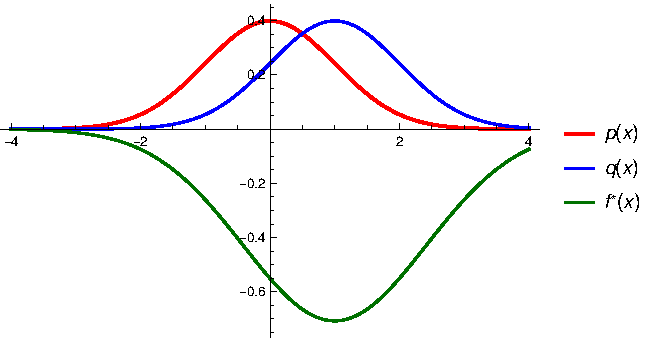
\includegraphics[scale=1.2]{../../presentation/img/s1.pdf}
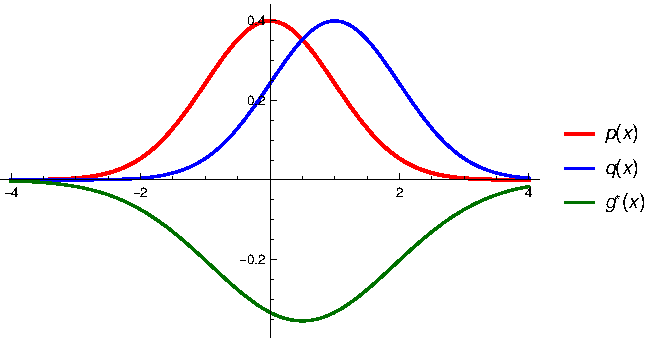
\includegraphics[scale=1.2]{../../presentation/img/s05.pdf}\\
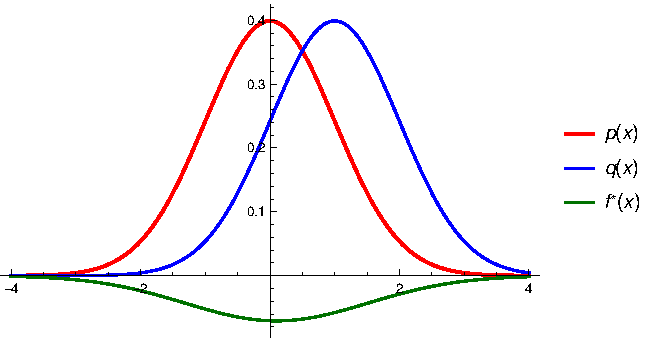
\includegraphics[scale=1.2]{../../presentation/img/s01.pdf}
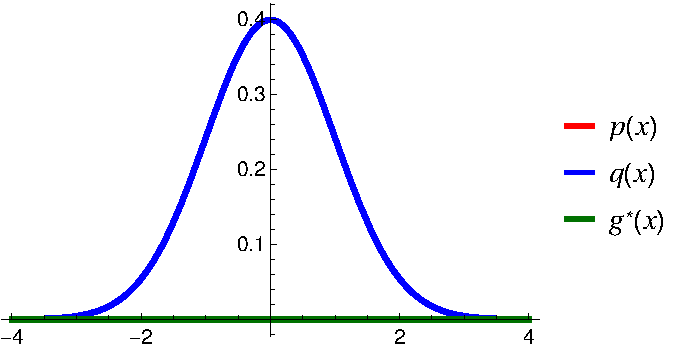
\includegraphics[scale=1.2]{../../presentation/img/s0.pdf}
\vspace{1cm}
\begin{center}
\emph{Bam!}
\end{center}
\end{block}



\vspace{-0.75cm}
\begin{block}{Closed form expression}
 Let $\mathcal{F}$ be the RKHS associated with the kernel $k$ and 
\large
 \begin{equation*}
\xi_{{ \color{red} p}}(x,\cdot):=\log' { \color{red} p}(x) k(x,\cdot)+  k'(x,\cdot).
\end{equation*}
 $\xi_{{ \color{red} p}}(x,\cdot)$ is an element of the reproducing kernel Hilbert
space $\mathcal{F}$.  $h$ is an  inner product between $\xi$, 
\[
h_{{\color{red} p}}(x,y)   = \langle\xi_{{ \color{red} p}}(x,\cdot),\xi_{{ \color{red} p}}(y,\cdot)\rangle. 
\]
$h$ can be written in close form
\large
\begin{align*}
h_{{\color{red} p}}(x,y) & = \partial_{x} \log {\color{red} p}(x) \partial_{x} \log {\color{red} p}(y) k(x,y)\\
 & \quad+\partial_{y} \log {\color{red} p}(y) \partial_{x}  k(x,y)\\
 & \quad+\partial_{x} \log {\color{red} p}(x) \partial_{y}k(x,y)\\
 & \quad+\partial_{x} \partial_{y} k(x,y).
\end{align*}
 \center{\emph{which only depends on kernel and $\partial_{x} \log {\color{red} p}(x)$}}
\end{block}

\vspace{-0.75cm}



 


\end{column}

%%%-----------------column 2
\hspace{-1.45cm}
\begin{column}{.33\linewidth}


\begin{block}{Theorem}
\large
Let ${ \color{blue} q},{\color{red} p}$ be probability measures and ${ \color{blue} Z}\sim { \color{blue} q}$. 
If $\ev_{{ \color{blue} q}} h_{{\color{red} p}}({ \color{blue} Z},{ \color{blue} Z})<\infty$, then 
$$MMD({\color{red} p},{ \color{blue} q},G) = \ev_{{ \color{blue} q}} h_{{\color{red} p}}({ \color{blue} Z},{ \color{blue} Z}'),$$
where ${ \color{blue} Z}'$ is an independent copy of ${ \color{blue} Z}$.
\end{block}

\vspace{-0.73cm}
\begin{block}{Proof}

Next we show that $\xi_{{ \color{red} p}}(x,\cdot)$ is Bochner integrable
\[
\ev_{{ \color{blue} q}}\|\xi_{{ \color{red} p}}({ \color{blue} Z})\|_{\mathcal{\mathcal{F}}}^{2}=\ev_{{ \color{blue} q}}h_{{ \color{red} p}}({ \color{blue} Z},{ \color{blue} Z})<\infty.
\]
We next relate the expected value of the Stein operator to the inner product of $f$ and the expected value
of $\xi_{{ \color{red} p}}({ \color{blue} Z})$,  
\begin{align*}
  \left\langle f,\ev_{{ \color{blue} q}} \xi_{{ \color{red} p}}({ \color{blue} Z}) \right\rangle _{\mathcal{\mathcal{F}}}& =\left\langle f,\ev_{{ \color{blue} q}} \left[  \log' { \color{red} p}({ \color{blue} Z}) k({ \color{blue} Z},\cdot)+\ k'({ \color{blue} Z},\cdot) \right] \right \rangle _{\mathcal{\mathcal{F}}}\\
 & = \ev_{{ \color{blue} q}}  \left\langle f,\left[  \log' { \color{red} p}({ \color{blue} Z}) k({ \color{blue} Z},\cdot)+\ k'({ \color{blue} Z},\cdot) \right] \right \rangle _{\mathcal{\mathcal{F}}}\\
 & =\ev_{{ \color{blue} q}}(T_{{ \color{red} p}}f)({ \color{blue} Z}).
\end{align*}
The second equality follows from  Bochner integrability of $\xi_{{ \color{red} p}}$.
We have 
\begin{align*}
MMD({ \color{red} p},{ \color{blue} q},G) & :=\sup_{\Vert f\Vert<1}\ev_{{ \color{blue} q}}(T_{{ \color{red} p}}f)({ \color{blue} Z})-\ev_{{ \color{red} p}}(T_{{ \color{red} p}}f)(X)\\
 & =\sup_{\Vert f\Vert<1}\ev_{{ \color{blue} q}}(T_{{ \color{red} p}}f)({ \color{blue} Z})\\
 & =\sup_{\Vert f\Vert<1}\langle f,\ev_{{ \color{blue} q}}\xi_{{ \color{red} p}}({ \color{blue} Z})\rangle_{{\cal \mathcal{F}}}\\
 & =\|\ev_{{ \color{blue} q}}\xi_{{ \color{red} p}}({ \color{blue} Z})\|_{\mathcal{\mathcal{F}}}.
\end{align*}
We now calculate closed form formula for $MMD({ \color{red} p},{ \color{blue} q},G)^{2}$,
\begin{align*}
MMD({ \color{red} p},{ \color{blue} q},G)^{2}  =\ev_{{ \color{blue} q}}\langle\xi_{{ \color{red} p}}({ \color{blue} Z}),\xi_{{ \color{red} p}}({ \color{blue} Z}')\rangle_{\mathcal{\mathcal{F}}}=\ev_{{ \color{blue} q}}h_{{ \color{red} p}}({ \color{blue} Z},{ \color{blue} Z}'),
\end{align*}
\end{block}


\vspace{-0.75cm}
\begin{block}{Theorem}
\vspace{1cm}


\large
If the kernel $k$ is $C_0$-universal, $\ev_{{ \color{blue} { \color{blue} q}}} h_{{ \color{blue} { \color{blue} q}}}({ \color{blue} Z},{ \color{blue} Z})<\infty$ and $\ev_{{ \color{blue} { \color{blue} q}}} (\log' \frac{{\color{red} p}({ \color{blue} Z})}{{ \color{blue} q}({ \color{blue} Z})})^{2}<\infty$
then $MMD({\color{red} p},{ \color{blue} q},G) =0$ if and only if ${\color{red} p}={ \color{blue} q}$.

\vspace{1cm}
\normalsize
Remarks.\\
Kernel is $C_0$-universal if  $f \to \int_X f(x) k(x,\cdot) d\mu(x)$ if is injective for all probability measures $\mu$ and all  $f \in L^p(X,\mu)$, where  $p \in [1,\infty] $. 
\vspace{0.5cm}

The assumption $\ev_{{ \color{blue} q}} (\log' \frac{{\color{red} p}({ \color{blue} Z})}{{ \color{blue} q}({ \color{blue} Z})})^{2}<\infty$ states that difference between scores $\log' \color{red} p$ and $\log' \color{blue} q$  is square integrable.
\end{block}

\vspace{-0.75cm}
\begin{block}{Proof}
 If ${ \color{red} p}={ \color{blue} q}$ then $MMD({\color{red} p},{ \color{red} p},G) =0$ is $0$. Suppose
${ \color{red} p}\neq { \color{blue} q}$, but $MMD({\color{red} p},{ \color{blue} q},G) =0$. If $MMD({\color{red} p},{ \color{blue} q},G) =0$ then, by Theorem 1 
$\ev_{{ \color{blue} q}}\xi_{{ \color{red} p}}({ \color{blue} Z})=0$. We substitute $\log { \color{red} p}({ \color{blue} Z})=\log { \color{blue} q}(Y)+[\log { \color{red} p}({ \color{blue} Z})-\log { \color{blue} q}(Y)]$,
\begin{align*}
 & \ev_{{ \color{blue} q}}\xi_{{ \color{red} p}}({ \color{blue} Z})\\
 & =\ev_{{ \color{blue} q}}\left( \log' { \color{red} p}({ \color{blue} Z})k({ \color{blue} Z},\cdot)+ k'({ \color{blue} Z},\cdot)\right)\\
 & =\ev_{{ \color{blue} q}}\xi_{{ \color{blue} q}}({ \color{blue} Z})+\ev_{{ \color{blue} q}}\left([\log { \color{red} p}({ \color{blue} Z})-\log { \color{blue} q}(Y)]'k({ \color{blue} Z},\cdot)\right)\\
 & =\ev_{{ \color{blue} q}}\left( [\log { \color{red} p}({ \color{blue} Z})-\log { \color{blue} q}(Y)]' k({ \color{blue} Z},\cdot)\right)
\end{align*}
The expected value of $(\log { \color{red} p}({ \color{blue} Z})-\log { \color{blue} q}({ \color{blue} Z}))' k({ \color{blue} Z},\cdot)$ is the mean embedding of
a function $g(y)=\left(\log\frac{{ \color{red} p}(y)}{{ \color{blue} q}(y)}\right)'$ with respect
to the measure ${ \color{blue} q}$.  $g$ is square integrable,
therefore, since the kernel $k$ is $C_0$-universal, %by \citet[ Theorem 4.4 c]{carmeli2010vector}
its embedding is zero if and only if $g=0$. This implies that 
\[
\log'\frac{{ \color{red} p}(y)}{{ \color{blue} q}(y)}=(0,\cdots,0).
\]
Consequently  $\log\frac{{ \color{red} p}(y)}{{ \color{blue} q}(y)}=C$, for some $C$, and so  ${ \color{red} p}(y)=e^{C}{ \color{blue} q}(y)$. Since ${ \color{red} p}$ and ${ \color{blue} q}$ both integrate
to one, $C=0$ then ${ \color{red} p}={ \color{blue} q}$, which is a contradiction.
\end{block}

\vspace{-0.75cm}
\begin{block}{Non i.i.d.\ extension: the wild bootstrap}
An estimator of $\ev h_{\color{red} p}(X,X')$ is  
\[
 V_n(h_{\color{red} p}) = \frac {1} {n^2} \sum_{i,j=1}^n h_{\color{red} p}(X_i,X_j).
\]
To estimate quantiles of $ V_n(h_{\color{red} p})$ we use wild bootstrap
\[
 B_n(h_{\color{red} p}) = \frac {1} {n^2} \sum_{i,j=1}^n W_i W_j h_{\color{red} p}(X_i,X_j).
\]
  where $W_i$ is a  series  random variables.
\begin{center}
  \begin{minipage}{.49\linewidth}
       $$
  Cov(W_i,W_j) = (1-2p_n)^{-|i-j|}
  $$
\end{minipage}
\begin{minipage}{.49\linewidth}
 \begin{figure}
            \vspace{-0.5cm}
           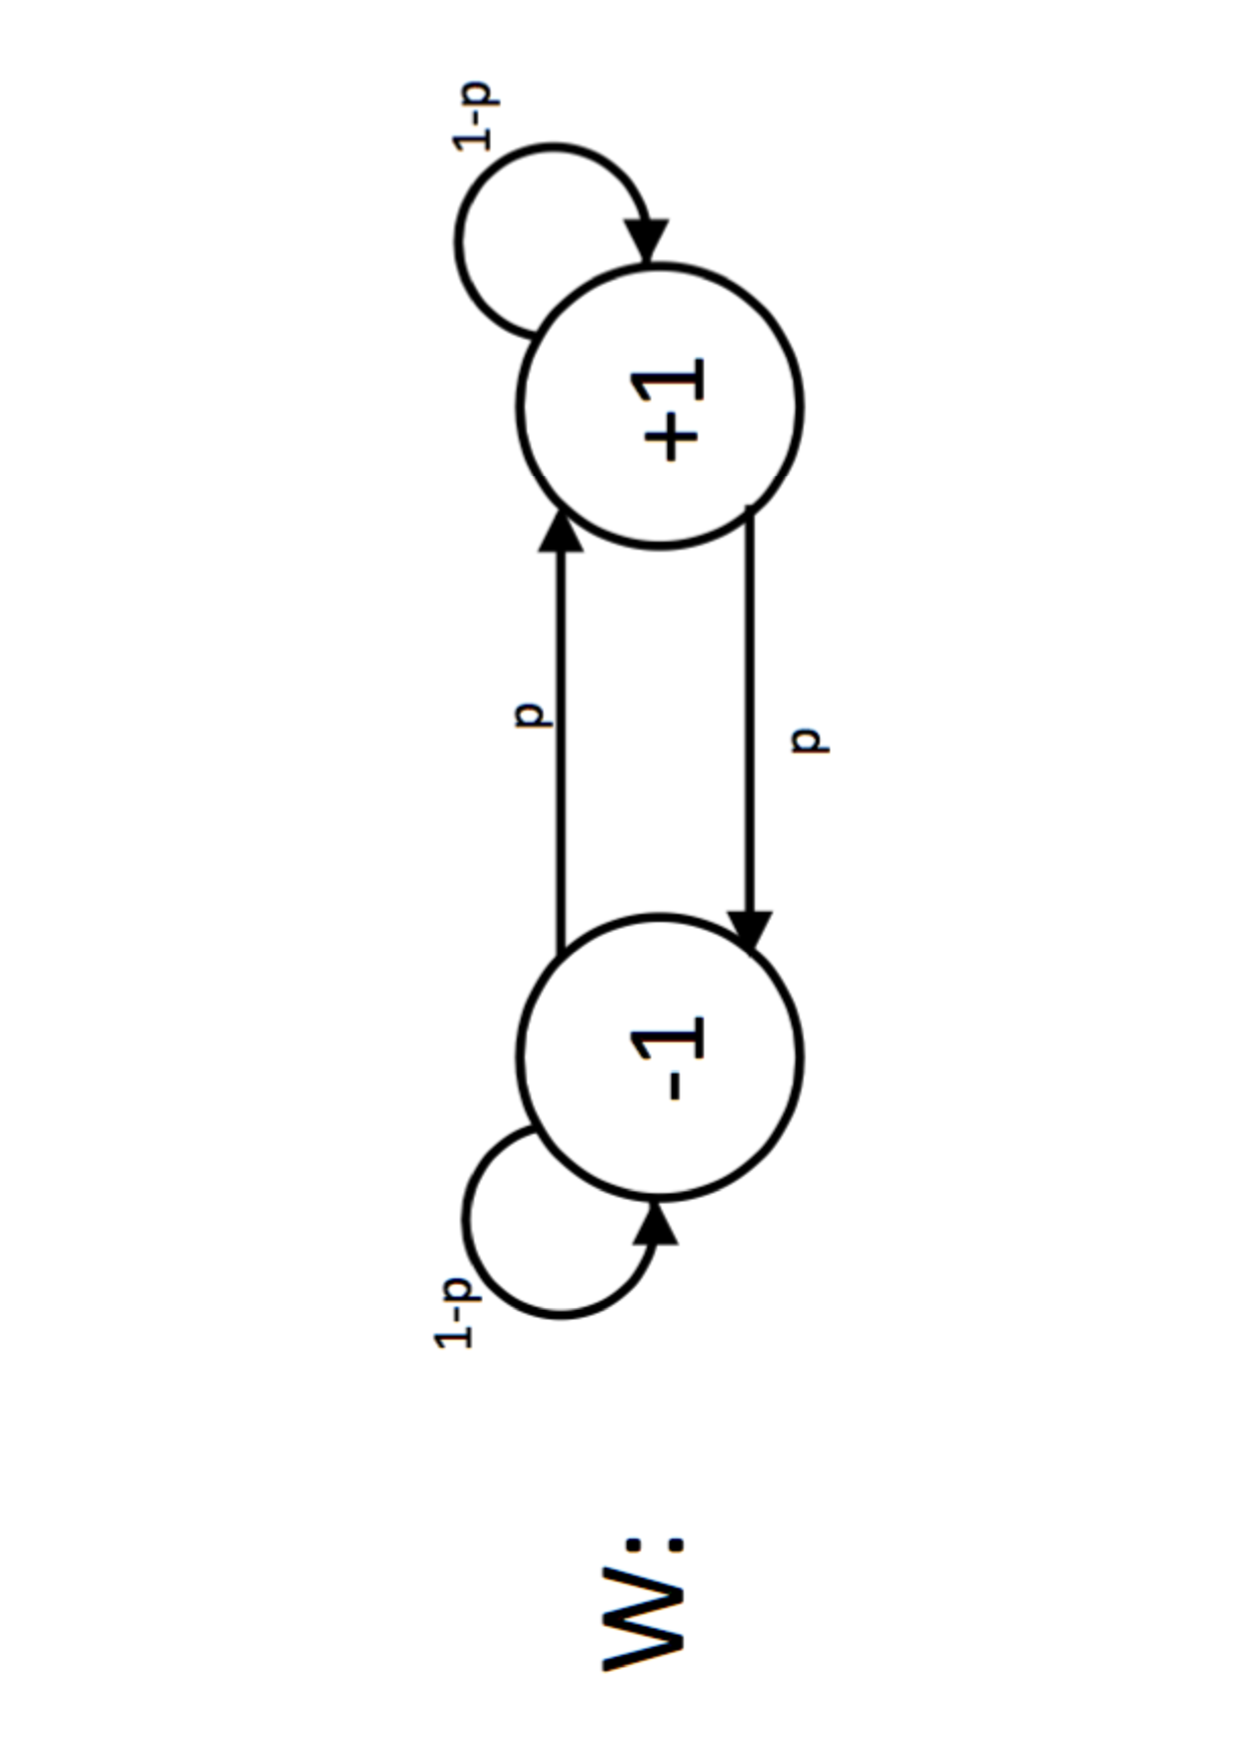
\includegraphics[width=0.7\textwidth, angle =0 ]{../../presentation/img/W_graphicalModel.pdf} 
        \end{figure}
\end{minipage}
\end{center}
  $p_n$ is  the probability of the change  and should be set to $o(n)$.

\setbeamertemplate{caption}{\raggedright\insertcaption\par}
\begin{center}

  \begin{minipage}{.49\linewidth}
\begin{figure}
 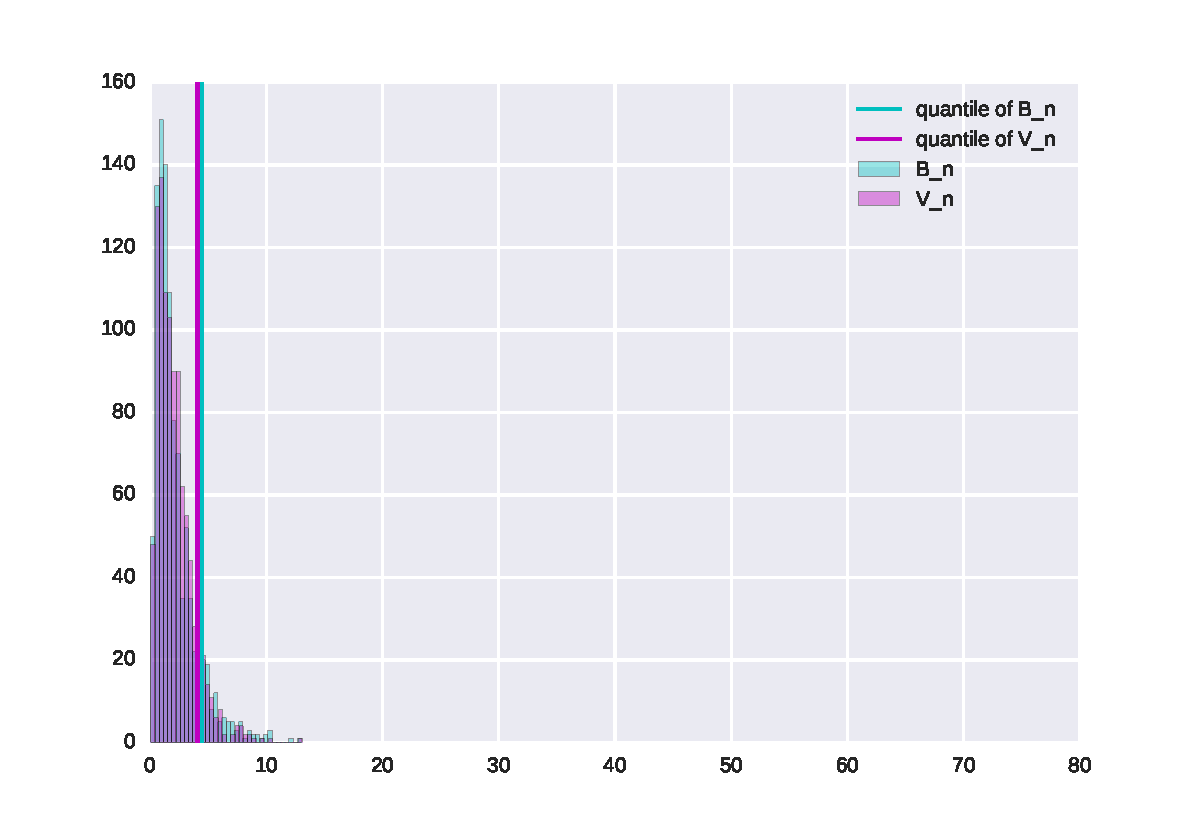
\includegraphics[width=\textwidth]{../../presentation/img/bootstrapWorks1.pdf}
 \caption{Small correlation in $W_t$} 
\end{figure}
 \end{minipage}
  \begin{minipage}{.49\linewidth}
\begin{figure}
 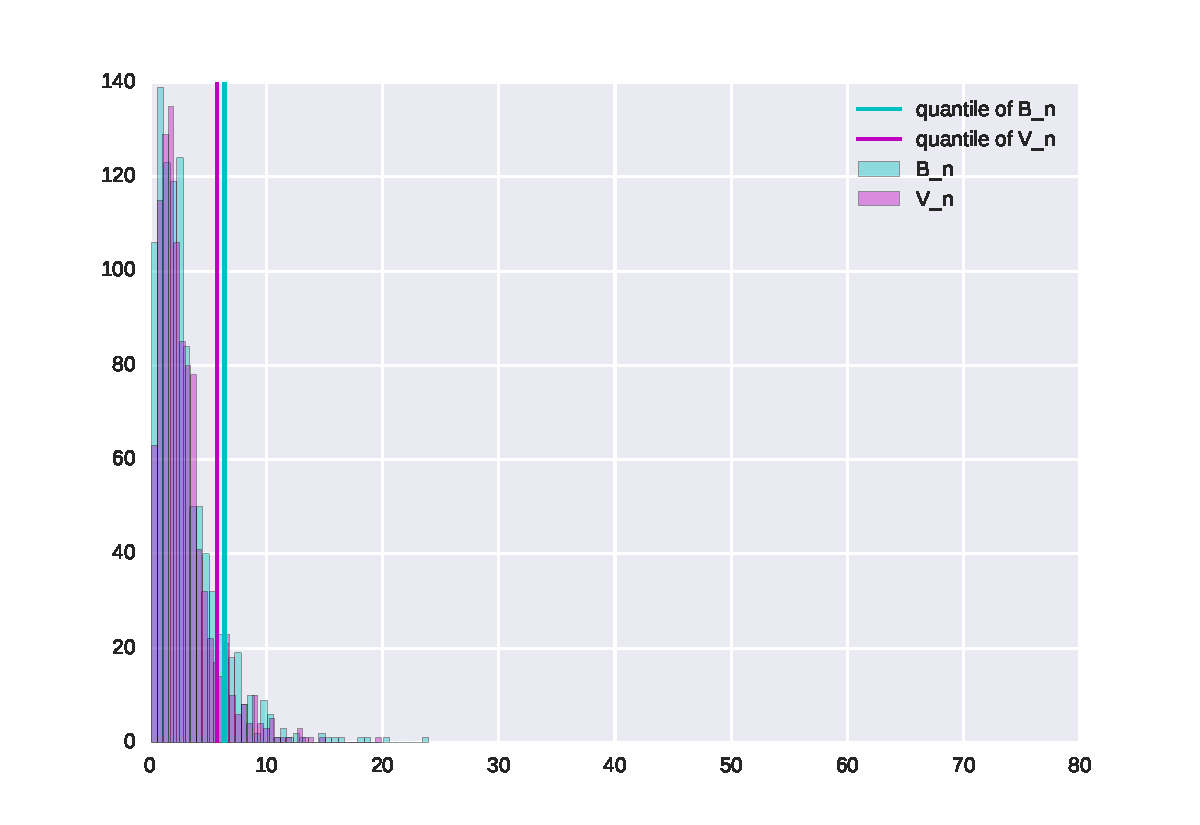
\includegraphics[width=\textwidth]{../../presentation/img/bootstrapWorks4.pdf}
 \caption{Medium correlation in $W_t$} 
\end{figure}
  \end{minipage}
\end{center}




 \begin{center}
  \begin{minipage}{.49\linewidth}
\begin{figure}
 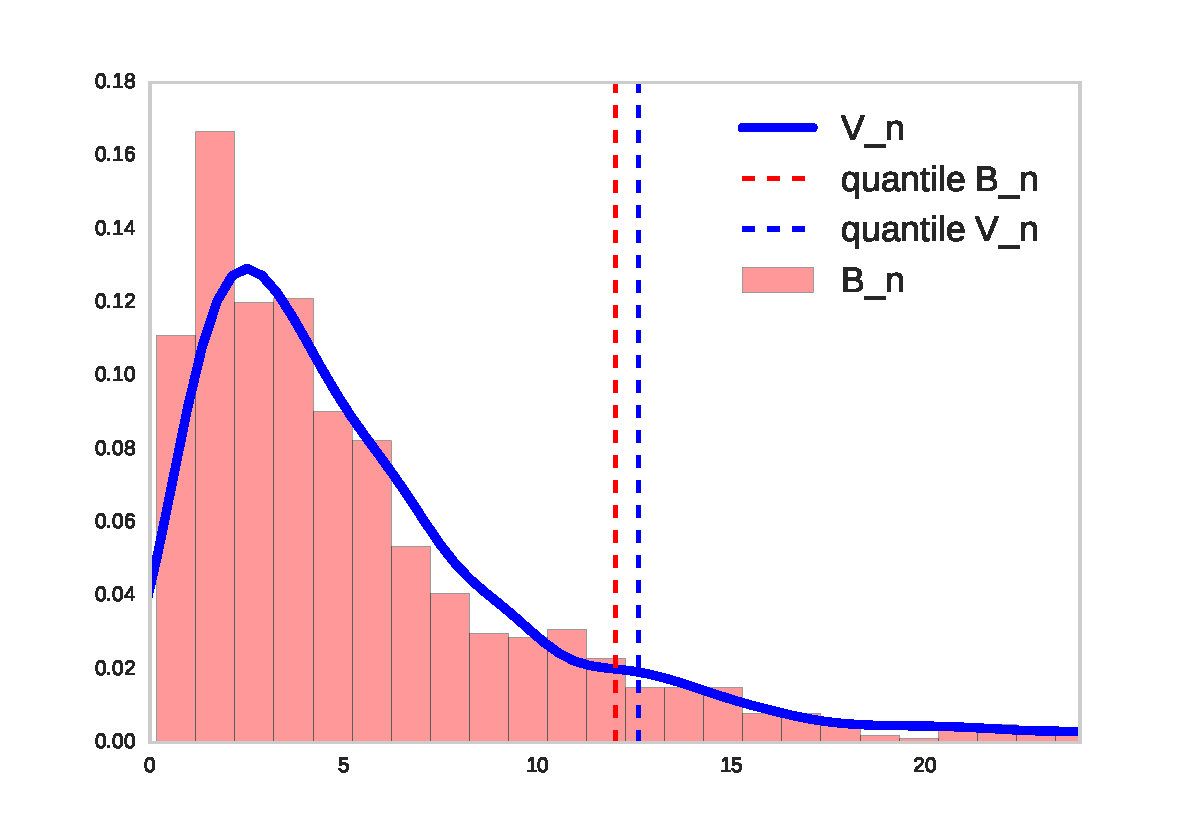
\includegraphics[width=\textwidth]{../../presentation/img/bootstrapWorks7.pdf}
 \caption{Brobdingnagian correlation in $W_t$} 
\end{figure}
  \end{minipage}
\begin{minipage}{.49\linewidth}
\begin{align*}
 X_t =& \beta X_{t-1} + \sqrt{1 - \beta^2}\epsilon_t\\
 & \epsilon_t \sim {\cal N}(0,1)
\end{align*}
 where $\beta$ controls the amount of autocorrelation in the process
\end{minipage}
\end{center}

 See also \cite{leucht_dependent_2013}.
\end{block}
\end{column}


% column 3
\hspace{-1.45cm}


\begin{column}{.32\linewidth}
%\vspace{-0.75cm}
\begin{block}{Consistency}
\large
 Suppose  $h$ is Lipschitz continuous and
$\ev h_{{ \color{red} p}}({ \color{blue} Z},{ \color{blue} Z})<\infty$. Under the null hypothesis $nV_n$ and $nB_n$ have the same limiting distribution (in a weak sense). Under the alternative hypothesis,
$B_{n}$ converges to zero, while $V_{n}$ converges to a positive
constant.

\end{block}


\vspace{-0.75cm}
\begin{block}{Experiment: Student's T vs.\ Normal}

\begin{center}
\begin{minipage}{.45\linewidth}
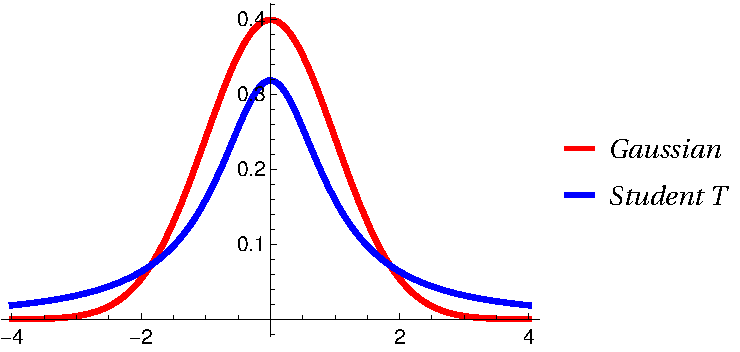
\includegraphics[width=\textwidth]{../../presentation/img/nt}
\end{minipage}
\begin{minipage}{.45\linewidth}
 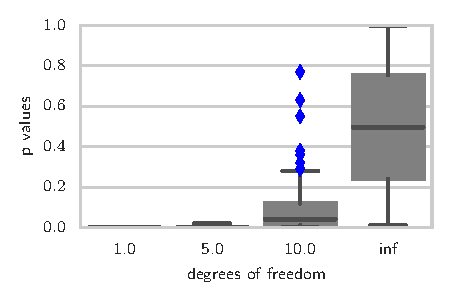
\includegraphics[width=\textwidth]{../../presentation/img/sgld_student_opt} 
\end{minipage}
\end{center}



We modify experiment 4.1 from \cite{gorham2015measuring} by  generating samples using
a Metropolis\textendash Hastings algorithm, with a Gaussian random walk with variance 1/2. We thin the observations by a factor of 20 and
set $a_{n}=0.1$, thus preserving both good statistical power and
correct calibration of p-values under the null hypothesis.

\end{block}
\vspace{-0.75cm}
\begin{block}{Experiment: Bias quantification in approximate MCMC}
E.g.\ \cite{korattikara2013austerity}
\begin{minipage}{.45\linewidth}
\begin{align*}
\theta_{1}\sim{\cal N}(0,10);\theta_{2}\sim{\cal N}(0,1)\\
X_{i}\sim\frac{1}{2}{\cal N}(\theta_{1},4)+\frac{1}{2}{\cal N}(\theta_{1}+\theta_{2},4) & .
\end{align*}

\end{minipage}
\begin{minipage}{.45\linewidth}
\begin{center}
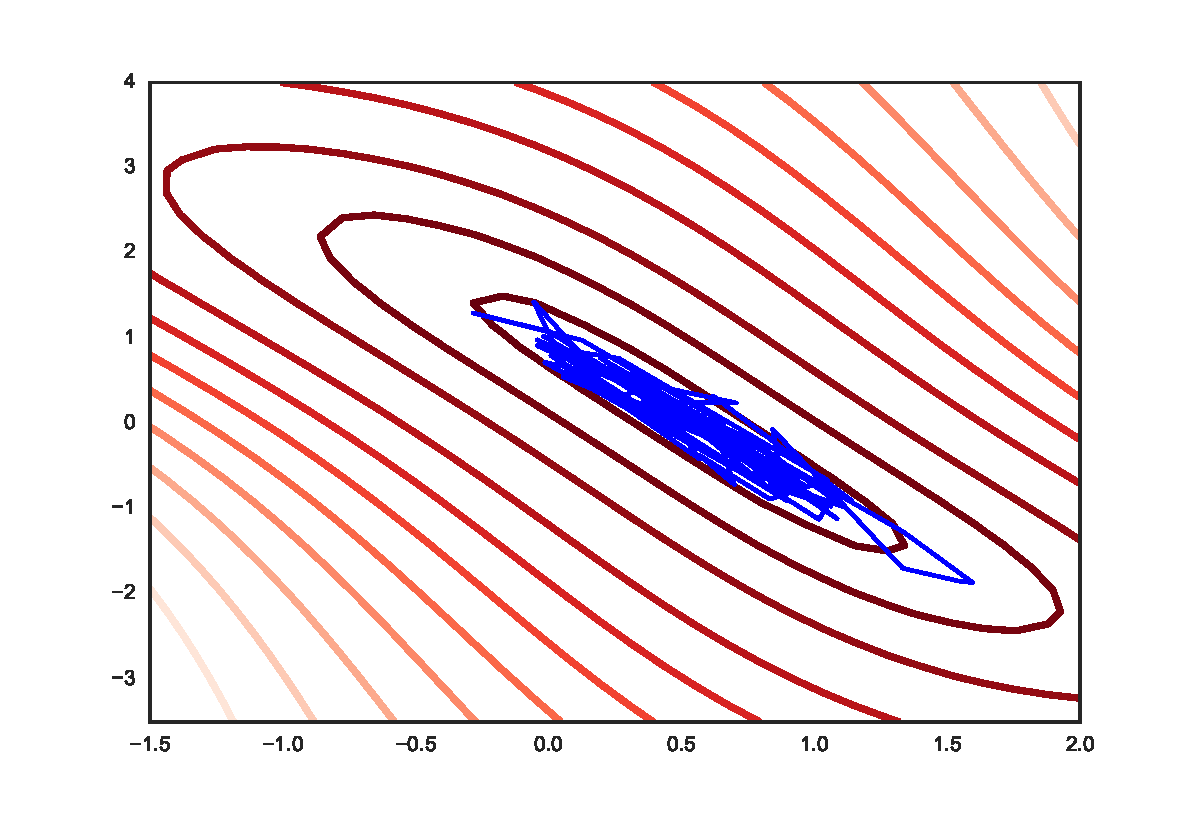
\includegraphics[width=0.5\textwidth]{../../presentation/img/sgld_trace_and_density.pdf}
\end{center}
\end{minipage}
\begin{minipage}{.450\linewidth}
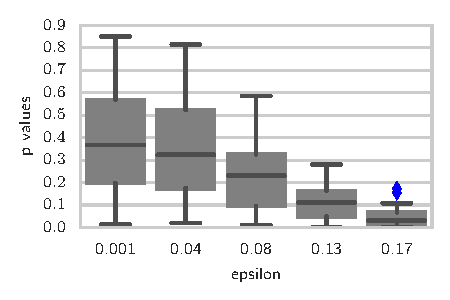
\includegraphics[width=.6\textwidth]{../../presentation/img/Heiko1}\\
\end{minipage}
\begin{minipage}{.45\linewidth}
            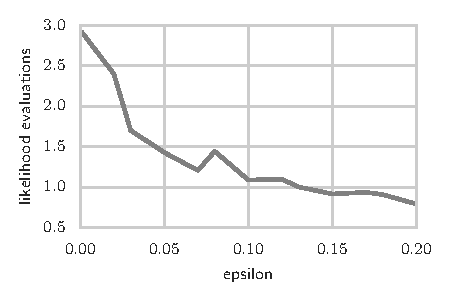
\includegraphics[width=.6\textwidth]{../../presentation/img/Heiko2}
\end{minipage}


\end{block}
\vspace{-0.75cm}
\begin{block}{Experiment: Statistical model criticism}
See \cite{lloyd2015statistical}.
\begin{center}
\item We test the hypothesis that a Gaussian process generated \textbf{training data} using for fitting -- without simulating from the generative model, but only using {\color{red} test data}.
\end{center}
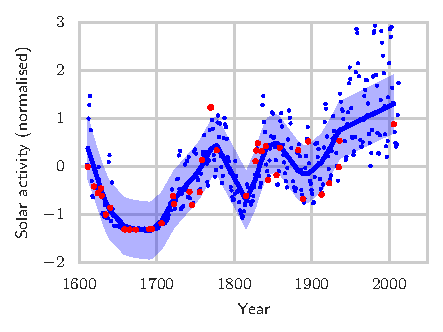
\includegraphics[width=0.48\textwidth]{../../presentation/img/gp_regression_data_fit.pdf} 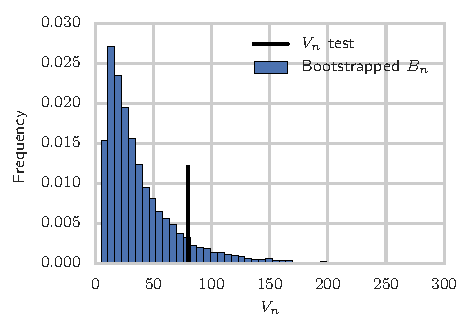
\includegraphics[width=0.48\textwidth]{../../presentation/img/gp_regression_bootstrap_hist} 
\begin{minipage}{.35\linewidth}

\end{minipage}
\end{block}
\begin{block}{Experiment: Convergence of density estimation}
\begin{center}
\item Tada
\end{center}
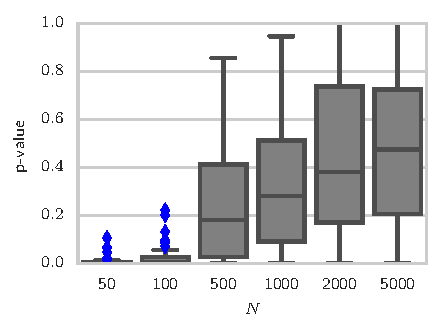
\includegraphics[width=0.48\textwidth]{../../presentation/img/increasing_data_fixed_test.pdf} 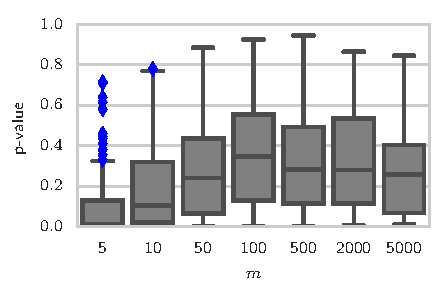
\includegraphics[width=0.48\textwidth]{../../presentation/img/increasing_features_fixed_test.pdf} 
\begin{minipage}{.35\linewidth}

\end{minipage}
\end{block}
\vspace{-0.75cm}
\begin{block}{References}


\begin{minipage}{.9\linewidth}
{\footnotesize
\begin{multicols}{2}
\setbeamertemplate{bibliography item}[text] 
\bibliographystyle{plain} 
\scriptsize
\bibliography{../../biblio.bib} \ 
\end{multicols}
} 
\end{minipage}
\end{block}

\end{column}
\end{columns}

\end{frame}
\end{document}
